\chapter{Практичні результати}

У четвертому розділі представлено практичні результати
застосування алгоритму дифузії з сегментацією
та без із зазначенням вхідних даних.

\section{Практичні результати}

Результати роботи програми зображені на рисунку \ref{fig:stereo:pixel}.
Зліва зображена карта глибин, отримана за допомогою алгоритму,
описаного в попередньому розділі, де кожній долі графа відповідає один піксель.
Справа зображена карта глибин,
отримана за допомогою об'єднання частин зображення в суперпікселі.

\begin{figure}[h]
  \centering
  \begin{subfigure}[b]{0.3\textwidth}
      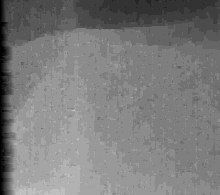
\includegraphics[width=\textwidth]{images/pixel_based_stereo}
      \caption{Карта глибин, отримана алгоритмом дифузії без застосування сегментації зображення}
  \end{subfigure}
  \begin{subfigure}[b]{0.3\textwidth}
      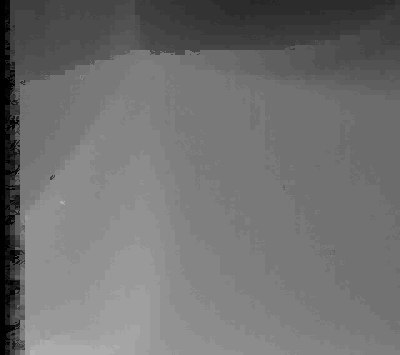
\includegraphics[width=\textwidth]{images/superpixel_based_stereo}
      \caption{Карта глибин, отримана алгоритмом дифузії після застосування сегментації зображення}
  \end{subfigure}
  \caption{Практичні результати}
  \label{fig:stereo:pixel}
\end{figure}

% TODO: launch pixel-based stereo with bigger smoothing term

Вхідні зображення (рис. \ref{fig:stereopair}) були взяті з набору зображень стереопар,
що були зроблені в Міддлберійскому коледжі в 2006 році
\cite{middlebury:ds:1} \cite{middlebury:ds:2}.

\begin{figure}[h]
  \centering
  \begin{subfigure}[b]{0.3\textwidth}
      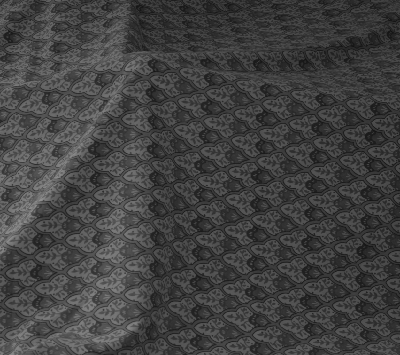
\includegraphics[width=\textwidth]{images/cloth_left_400}
      \caption{Ліве зображення стереопари}
  \end{subfigure}
  \begin{subfigure}[b]{0.3\textwidth}
      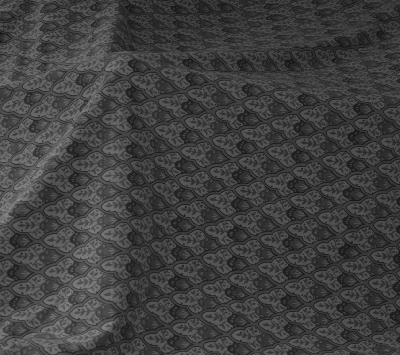
\includegraphics[width=\textwidth]{images/cloth_right_400}
      \caption{Праве зображення стереопари}
  \end{subfigure}
  \caption{Вхідні зображення}
  \label{fig:stereopair}
\end{figure}

Програмне забезпечення
було написано на мові програмування Rust спеціально для цієї роботи.

% Такого результату вдалося досягти за $524$ мілісекунди на компьютері з
% процесором Intel Core i5-3317U, виконавши $28$ ітерацій алгоритму.
% Програмне забезпечення будо написано на Pyhton $2.7$ спеціально для цієї роботи.

\section*{Висновки до розділу 4}
\addcontentsline{toc}{section}{Висновки до розділу 4}
